\documentclass[12pt]{report}

\usepackage[brazilian]{babel}
\usepackage[utf8]{inputenc}
\usepackage[top=1 in,bottom=1in, left=1 in, right=1 in]{geometry}

%Some packages I commonly use.
\usepackage{graphicx}
\usepackage{amsmath}
\usepackage{amsthm}
\usepackage{amssymb}
\usepackage{amsfonts}
\usepackage{natbib}
\usepackage{enumerate}
\usepackage{xcolor}
\usepackage{dashrule}
\usepackage{xfrac}
\usepackage{cancel}
\usepackage{multirow}
\usepackage{hyperref}



\usepackage{mathtools}	% text over arrow

%A bunch of definitions that make my life easier
\newcommand{\comment}[1]{}
\newcommand{\ds}{\displaystyle}

% definitions
\newcommand{\basis}{\varphi}
\newcommand{\mult}{\lambda}    % lagrange multiplier
\newcommand{\Mult}{\bm{\Lambda}}    % lagrange multiplier solutions
\newcommand{\multt}{\mu}       % lagrange multiplier test function
% \newcommand{\edges}{\varepsilon^\Omega}
\newcommand{\edgessymbol}{\mathcal{E}}
\newcommand{\edges}{{\edgessymbol^\Omega}}
\newcommand{\edgesinner}{\edgessymbol^\Omega_0}
\newcommand{\edgesboundary}{{\edgessymbol^\Omega_\Gamma}}

% operators
\renewcommand{\div}{\mathrm{div}\,}
\newcommand{\grad}{\nabla}
\newcommand{\rot}{\text{rot}\,}
% \DeclareMathOperator{\adj}{adj}
\newcommand{\erf}{\mathrm{erf}}
\renewcommand{\d}{\partial}
\newcommand{\inner}[2]{{\left\langle {#1}, {#2} \right\rangle}}
\newcommand{\jump}[1]{{\llbracket {#1} \rrbracket}}
\newcommand{\argmin}{\operatornamewithlimits{argmin}}


% spaces
\newcommand{\R}{\mathbb{R}}
\renewcommand{\P}{\mathbb{P}}
\newcommand{\Hs}{\mathcal{H}}
\newcommand{\Ls}{\mathcal{L}}
\newcommand{\Vs}{\mathcal{V}}
\newcommand{\Qs}{\mathcal{Q}}
\newcommand{\Hdiv}{\Hs(\text{div})}
\newcommand{\Hrot}{\Hs(\text{rot})}

% matrices
\newcommand{\M}{\mathbf{M}}
\newcommand{\A}{\mathbf{A}}
\newcommand{\B}{\mathbf{B}}
\newcommand{\C}{\mathbf{C}}
\renewcommand{\H}{\mathbf{H}}
\renewcommand{\L}{\mathbf{L}}
\newcommand{\G}{\mathbf{G}}
\newcommand{\U}{\mathbf{U}}
\renewcommand{\P}{\mathbf{P}}
% global matrices
\renewcommand{\AA}{\tilde{\A}}
\newcommand{\BB}{\tilde{\B}}
\newcommand{\CC}{\tilde{\C}}
\newcommand{\UU}{\tilde{\U}}
\newcommand{\HH}{\tilde{\H}}
\newcommand{\K}{\mathbf{K}}
\newcommand{\X}{\mathbf{X}}
\newcommand{\F}{\mathbf{F}}

% vectors
\newcommand{\x}{\mathbf{x}}
\renewcommand{\u}{\mathbf{u}}
\renewcommand{\v}{\mathbf{v}}
\newcommand{\n}{\mathbf{n}}

% integrals over domain
\newcommand{\intD}[1]{\int_{\Omega} \,{#1}\, \mathrm{d} \x}
\newcommand{\intDk}[1]{\int_{\Omega_k} \,{#1}\, \mathrm{d} \x}
\newcommand{\intC}[1]{\int_{\Gamma} \,{#1}\, \mathrm{d} s}
\newcommand{\intCk}[1]{\int_{\Gamma_k} \,{#1}\, \mathrm{d} s}
\newcommand{\intCD}[1]{\int_{\Gamma_D} \,{#1}\, \mathrm{d} s}
\newcommand{\intCN}[1]{\int_{\Gamma_N} \,{#1}\, \mathrm{d} s}



% multiphase model
\newcommand{\sa}{S_\alpha}
\newcommand{\sar}{S_{\alpha r}}
\newcommand{\ka} {k_\alpha}
\newcommand{\kra}{k_{r \alpha}}
\newcommand{\la} {\lambda_\alpha}
\newcommand{\mua}{\mu_\alpha}
\newcommand{\fa} {f_\alpha}
\newcommand{\ua} {\u_\alpha}
\newcommand{\va} {\v_\alpha}
\newcommand{\ma} {m_\alpha}
\newcommand{\rhoa} {\rho_\alpha}
\newcommand{\Va} {V_\alpha}
\newcommand{\gradpa} {\gradp_\alpha}

\renewcommand{\k}{\mathbf{k}}
\newcommand{\lo}{\lambda_{o}}
\newcommand{\lw}{\lambda_{w}}
\newcommand{\muo}{\mu_o}
\newcommand{\muw}{\mu_w}
\newcommand{\kro}{k_{ro}}
\newcommand{\krw}{k_{rw}}
\newcommand{\sw}{S_w}
\newcommand{\swc}{S_{wc}}
\newcommand{\sor}{S_{or}}
\newcommand{\so}{S_o}
\newcommand{\uo}{u_o}
\newcommand{\uw}{u_w}
\newcommand{\gradp}{\nabla p}
\newcommand{\pc}{p_c}
\newcommand{\fw}{f_w}
\newcommand{\fo}{f_o}


% unities
\newcommand{\upsi}{\,\mathrm{psi}}
\newcommand{\uft}{\,\mathrm{ft}}
\newcommand{\uPa}{\,\mathrm{Pa}}
\newcommand{\um}{\,\mathrm{m}}

% fractions utilities
\newcommand{\pfrac}[2]{\left( \frac{#1}{#2} \right)}			% fraction between parenthesis
\newcommand{\bfrac}[2]{\left[ \frac{#1}{#2} \right]}			% fraction between brackets
\newcommand{\diff}[2]{\frac{\mathrm{d} #1}{\mathrm{d} #2}}		% fraction for derivative
\newcommand{\pdiff}[2]{\frac{\partial #1}{\partial #2}}		% fraction for partial derivative

% coloring
% \usepackage[dvipsnames]{xcolor}
\newcommand{\red}[1] {{\color {red}#1}}
\newcommand{\blue}[1]{{\color{blue}#1}}
\newcommand{\green}[1]{{\color{PineGreen}#1}}
\newcommand{\gray}[1]{{\color{gray}#1}}
\newcommand{\hdline}{{\color{gray} \hdashrule[0.5ex]{\textwidth}{1pt}{1mm}}}


%\numberwithin{equation}{chapter}

\title{Roteiro completo e entendível de \\Métodos de Elementos Finitos}
\author{Jhuan Cedro}
%\date{January 2019}

\begin{document}
\maketitle
\tableofcontents
\newpage

	
\chapter{Introdução}	
\label{c:introducao}
.

\chapter{Essencial do cálculo?}
	\red{ Só relembrar umas coisas bem básicas e deixar muitas referências
	\begin{itemize}
		\item O que é divergente, gradiente, jacobiana, hessiana;
		\item Problemas de otimização de funções diferenciáveis;
		\item Integração por partes, teorema de Green e Gauss;
		\item (\textbf{álgebra linear}) Espaço vetorial, base, distância e norma.
	\end{itemize}
	}

\chapter{Método dos Mínimos Quadrados}
	Os métodos de elementos finitos tem o objetivo de aproximar a solução de um problema diferencial por funções mais simples. Nessa linha, eles acabam recaindo em um método que tem o mesmo princípio, mas sem a parte diferencial. Apresentamos aqui a ideia do método de mínimos quadrados, pois ela será bem útil adiante.
	
	Suponha que você possui um conjunto de dados ... \red{Achar exemplo e figura} (\red{com $N$ pontos})
	\begin{figure}[h!]
		\centering
		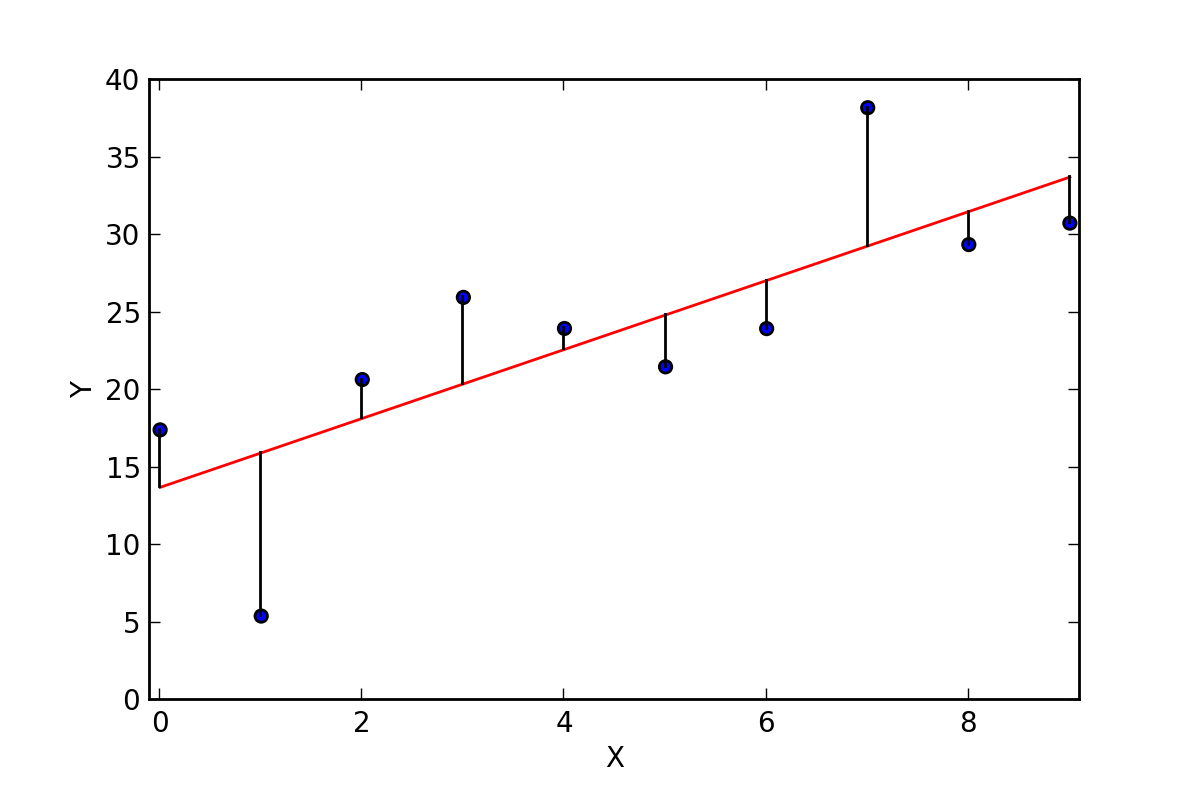
\includegraphics[width=0.5\linewidth]{img/minimos-quadrados-erros.png}
		\caption{... 
%		\footnote{https://upload.wikimedia.org/wikipedia/commons/e/ed/Residuals\_for\_Linear\_Regression\_Fit.png} 
		}
	\end{figure}
	
	Imagine que você queira encontrar uma função que descreve \red{os seus dados}. Porém, as observações nem sempre são precisas e podem conter erros. Além disso, pode ser que a função que você escolha pra representar seus dados não seja perfeita. Você pode escolher uma reta, uma equação do segundo grau, uma curva exponencial, e por aí vai. O método de mínimos quadrados se propõe a encontrar a função $f(x)$ que \textbf{melhor se aproxime} dos seus dados $y(x)$, \textbf{dentro de um conjunto de funções} de sua escolha.
	
	Por exemplo, se você quiser encontrar a melhor reta que aproxima $y(x)$, você quer escolher $f(x)$ dentro do conjunto de polinômios de primeiro grau. Qualquer polinômio de primeiro grau pode ser escrito como:
	\begin{equation*}
		p_1(x) = ax + b
		\,, \quad \forall \, a, b \in \R.
	\end{equation*}
	\blue{
	Portanto, podemos definir o conjunto de todos os polinômios de primeiro grau como:
	\begin{equation}
		\mathbb{P}_1 = \left\{ p : \R \rightarrow \R \;\big|\; p(x) = ax + b \,, \forall a, b \in \R \right\} 
	\end{equation}
	}
	
	Então, nossa missão é encontrar $a$ e $b$, de forma que $f(x)=p_1(x)$ seja a melhor aproximação possível de $y(x)$. Porém, precisamos definir que é ser melhor. Fazemos isso definindo o quanto uma função $f$ erra ao tentar aproximar $y$. Por exemplo, em um ponto $x_i$ o valor da sua função deveria ser $y_i$, mas na verdade é $f(x_i)$. Essa diferença entre o real e o aproximado é o que chamamos de erro:
	\begin{equation}
		\text{erro de $f$ no ponto $i$} 
		%= \mathrm{erro_i} 
		= y_i - f(x_i) \,.
	\end{equation}
	Essa forma de definir erro tem a desvantagem de existirem erros positivos e negativos. Como para nós é tudo erro, o sinal não interessa. Nesse método, consideraremos o erro quadrático, definido por:
	\begin{equation}
		\text{erro quadrático de $f$ no ponto $i$} 
		%= \mathrm{erro_i} 
		= (y_i - f(x_i))^2 \,.
	\end{equation}
	
	Definimos a melhor função $f$ como aquela que tem a menor soma dos erros quadráticos em todos os $N$ pontos. Assim, temos um problema de \textbf{minimização funcional}, onde:
	\begin{equation}
		f = \text{polinômio $p_1$ que minimize}		
		\;\sum_{i=1}^{N} \big(y_i - p_1(x_i) \big)^2
		%\min_{f \in \mathbb{P}_1}\sum_{i=1}^{N}(y_i - f(x_i))^2
	\end{equation}

\color{blue}	
	Mais formalmente:
	\begin{equation}
		f =  \argmin_{p_1 \,\in\, \mathbb{P}_1} \sum_{i=1}^{N}(y_i - p_1(x_i))^2
	\end{equation}
	Como sabemos que $p_1(x)=ax+b$, e também conhecemos todos os pontos $x_i$ e $y_i$, podemos afirmar que o erro total depende apenas de $a$ e $b$, ou seja:
	\begin{equation}
		\mathrm{Erro}(a, b) = E(a, b) = \sum_{i=1}^{N}(y_i - p_1(x_i))^2 = \sum_{i=1}^{N}(y_i - (a x_i + b))^2
	\end{equation}
	
	Por sorte, sabemos cálculo! Então sabemos que o ponto mínimo da função $\text{Erro}(a, b)$ ocorre, necessariamente, quando:
	\begin{equation*}
		\pdiff{E}{a} = 0 \qquad \text{e} \qquad \pdiff{E}{b} = 0 
%		\,, \qquad 
%		\pdiff{^2 E}{a^2} > 0
%		\, \qquad \text{e} \qquad
%		\pdiff{^2 E}{b^2} > 0
		\,.
	\end{equation*}
		
%	Comecemos pela regra da derivada primeira. 
	Como o erro é um somatório, e sabemos que a derivada da soma é a soma das derivadas, temos:
	\begin{equation}
	\begin{split}
		\ds \pdiff{E}{a} 
			&= \ds \pdiff{}{a} \left[ \sum_{i=1}^{N}(y_i - (a x_i + b))^2 \right]
			 = \ds \sum_{i=1}^{N} \pdiff{}{a} \Big[ (y_i - a x_i - b)^2 \Big]
			 = \ds \sum_{i=1}^{N} \Big[ 2 (y_i - a x_i - b) (-x_i) \Big]
			 \\
			&= \ds 2\, \sum_{i=1}^{N} \Big[ - x_i y_i + a x_i^2 +  bx_i  \Big] = 0
			\quad \longrightarrow \quad
			 a \sum_{i=1}^{N} x_i^2 + b \, \sum_{i=1}^{N} x_i   = \sum_{i=1}^{N} (x_i y_i)
		\\ \ds
	\end{split}
	\end{equation}
	
	\gray{
	\begin{equation}
	\begin{split}
		\ds \pdiff{E}{a} 
			&= \ds \pdiff{}{a} \left[ \sum_{i=1}^{N}(y_i - p_1(x_i))^2 \right]
		 = \ds \sum_{i=1}^{N} \pdiff{}{a} \Big[ (y_i - p_1(x_i))^2 \Big]
		 = \ds \sum_{i=1}^{N} \left[ 2 p_1(x_i) \pdiff{p_1(x_i)}{a} \right]
		\\ \ds
	\end{split}
	\label{e:mmq-exemplo1-1}
	\end{equation}
	}
	
	\begin{equation}
	\begin{split}
		\ds \pdiff{E}{b} 
			&= \ds \pdiff{}{b} \left[ \sum_{i=1}^{N}(y_i - (a x_i + b))^2 \right]
			 = \ds \sum_{i=1}^{N} \pdiff{}{b} \Big[ (y_i - a x_i - b)^2 \Big]
			 = \ds \sum_{i=1}^{N} \Big[ 2 (y_i - a x_i - b) (-1) \Big]
			 \\
			&= \ds 2 \, \sum_{i=1}^{N} \Big[ - y_i + a x_i + b \Big] = 0
			\quad \longrightarrow \quad
			a\, \sum_{i=1}^{N} x_i + b\, \sum_{i=1}^{N} 1 = \sum_{i=1}^{N} y_i
	\end{split}
	\label{e:mmq-exemplo1-2}
	\end{equation}
	
	Juntando \eqref{e:mmq-exemplo1-1} e \eqref{e:mmq-exemplo1-2} podemos escrever o sistema matricial:
	\begin{equation}
		\setlength\arraycolsep{8pt}
		\begin{bmatrix}
			\ds \sum_{i=1}^{N} x_i^2 	& \ds \sum_{i=1}^{N} x_i \\[20pt]
			\ds \sum_{i=1}^{N} x_i 		& \ds N %\sum_{i=1}^{N} 1
		\end{bmatrix}
		\begin{bmatrix}
			a \\[20pt] b
		\end{bmatrix}
		=
		\begin{bmatrix}
			\ds \sum_{i=1}^{N} x_i y_i \\[20pt]
			\ds \sum_{i=1}^{N} y_i
		\end{bmatrix}
		\label{e:mmq:exemplo1-3}
	\end{equation}
	
	Satisfazer o sistema assim é uma \textbf{condição necessária} para que um ponto $(a, b)$ seja mínimo da função $E(a, b)$, mas ainda \textbf{não garante} que este ponto seja um mínimo local de $E$ (menos ainda que seja global). Para garantir que encontramos um ponto $(a, b)$ que minimize o erro, devemos olhar para as propriedades da matriz hessiana e da convexidade de $E$. Para não nos estendermos demais, assumiremos apenas que a solução de \eqref{e:mmq:exemplo1-3} minimiza o erro $E$. Mais detalhes podem ser encontrados em \ref{...}.
	
	Note que a escolha da função de erro é fundamental para o funcionamento do método. Poderíamos ter pensado em escolher o erro de $f$ num ponto $x_i$ como sendo, por exemplo, $|y_i-f(x_i)|$. Contudo, não teríamos uma função diferenciável (a função módulo tem ``bicos'') e não poderíamos aplicar essa tática de minimização, baseada em derivadas, que apresentamos.

\gray{	
	Só pra garantir, vamos ver a \textbf{hessiana}:
	\begin{equation}
		\begin{split}
		\ds \pdiff{^2 E}{a^2} 
			%= \ds \pdiff{}{a} \left[ \pdiff{E}{a} \right]
			&= \ds \pdiff{}{a} \left[ 2 \, \sum_{i=1}^{N} (-x_i y_i + a x_i^2 + bx_i) \right]
			 = \ds 2 \, \sum_{i=1}^{N} x_i^2
		\\
		\ds \pdiff{}{a} \pdiff{E}{b} = \pdiff{}{b} \pdiff{E}{a}
			%= \ds \pdiff{}{b} \left[ \pdiff{E}{a} \right]
			&= \ds \pdiff{}{b} \left[ 2 \, \sum_{i=1}^{N} (-x_i y_i + a x_i^2 + bx_i) \right]
			 = \ds 2 \, \sum_{i=1}^{N} x_i
		\\
		\ds \pdiff{^2 E}{b^2} 
			%= \ds \pdiff{}{a} \left[ \pdiff{E}{a} \right]
			&= \ds \pdiff{}{b} \left[ 2 \, \sum_{i=1}^{N}  (- y_i + a x_i + b) \right]
			 = \ds 2N
		\end{split}
	\end{equation}
	
	\begin{equation}
		\mathbf{H}_E = 
		2 
		\begin{bmatrix}
			\ds \sum_{i=1}^{N} x_i^2 & \ds \sum_{i=1}^{N} x_i \\[15pt]
			\ds \sum_{i=1}^{N} x_i   & \ds N
		\end{bmatrix}
		\quad \rightarrow \quad
		\det \mathbf{H}_E = 2 \left[ N \sum_{i=1}^{N} x_i^2 + \left( \sum_{i=1}^{N} x_i \right)^2 \right] \ge 0
	\end{equation}
	
	Caso exista ao menos um ponto $x_i \neq 0$, então podemos afirmar que $\det \mathbf{H}_E > 0$. Segundo Diva Flemming, se $\det \mathbf{H}_E > 0$ e $\pdiff{^2 E}{a^2}$ em um ponto $(a, b)$, então este ponto é um mínimo local de $E$. 
	\red{Se $E$ for convexa ($\mathbf{H}_E$ é positiva semi-definida), garantimos que esse mínimo é global.
	
	\textbf{Essa parte da Hessiana pode ficar de fora, ou ir para algum apêndice.} Até porque, se for provar pro caso geral vai ser um inferno.}
}
		
\color{black}
	\textbf{Partiu falar do caso geral?}
	
	


\red{
	\begin{itemize}
	\item O que são resíduos ponderados?
	\item O que são métodos de regressão? 
	\item Falar de projeção e espaços
	\end{itemize}
}

\chapter{Interpolação}
\section{Interpoladores de Lagrange}

\chapter{Problema exemplo I}
\section{Formulação fraca}
	\red{O que é projeção e o que é formulação variacional?}
\section{Aproximação polinomial}
\section{Elemento de referência}
	\red{Qual o melhor momento pra falar disso? Primeiro dá um exempli e depois estende com jacobiana e tudo mais?}

\chapter{Métodos de Elementos Finitos}
\label{c:elementos-finitos}
Métodos de elementos finitos são técnicas numéricas para a resolução de equações diferenciais estacionárias. Estas consistem principalmente na discretização do domínio físico do problema em diversos subdomínios (elementos) sobre os quais são obtidas aproximações para a solução do problema \cite{Zienkiewicz00}.

Na Figura \ref{f:mef-discretizacao} é mostrado o exemplo de uma discretização de um domínio unidimensional $\Omega$ em quatro subdomínios $\Omega_{e_1}$ a $\Omega_{e_4}$. Nesta Figura, é representada a solução $u$ do problema em questão.

\begin{figure}[h!]
	\centering
	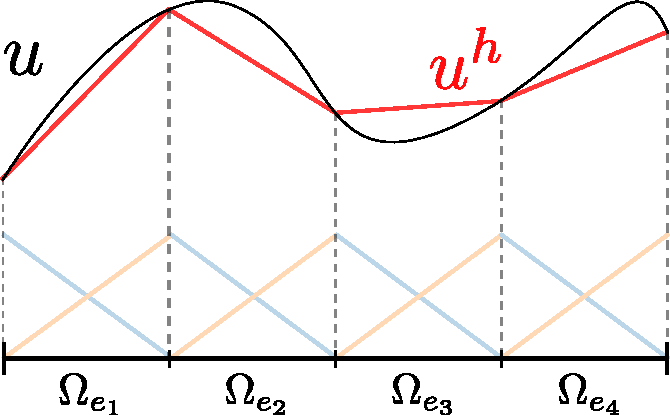
\includegraphics[width=0.5\linewidth]{img/dominio-solucao1}
	\caption{Exemplo de discretização de um domínio unidimensional $\Omega = \bigcup_{i=1}^4 \Omega_{e_i}$, onde $u$ é a solução analítica do problema e $u_h$ é a solução aproximada por um método de elementos finitos.}
	\label{f:mef-discretizacao}
\end{figure}

A aproximação de $u$, denotada por $u_h$, é obtida a partir da combinação linear de funções de uma base definida em cada subdomínio $\Omega_{e_i}$. Frequentemente são adotadas funções polinomiais, mais especificamente, bases de Lagrange. No exemplo da Figura \ref{f:mef-discretizacao} são mostradas, em azul e laranja, bases do espaço de polinômios lineares. 

Os polinômios de uma base de Lagrange de ordem $p$ são obtidos a partir de $p+1$ pontos de referência do domínio ($x_i$, $i\in[1, p+1]$). A base é constituída por $p+1$ polinômios $\phi_i^p(x)$ definidos por \eqref{e:lagrange}.

\begin{equation}
	\begin{array}{rc}
	\multirow{2}{*}{$
		\displaystyle
		\phi_i^p(x) = \prod_{j=1, j \neq i}^{p+1} \frac{x-x_j}{x_i-x_j}
		$,} &
	x_a \neq x_b \Leftrightarrow  a \neq b \\ & 
	1 \leq i, j \leq p+1
	
	\end{array}
	\label{e:lagrange}
\end{equation}

As Figuras \ref{f:lagrange-p1} a \ref{f:lagrange-p3} ilustram as funções de Lagrange para algumas ordens de polinômios. Cabe observar que $\phi^p_i(x_j)$ é unitário se $i=j$ e nulo se $i \neq j$. Bases de ordens mais altas apresentam maior capacidade de aproximar a solução, possibilitando a melhoria das aproximações pelo que se denomina refinamento $p$. 

\begin{figure}[h!]
	\centering
	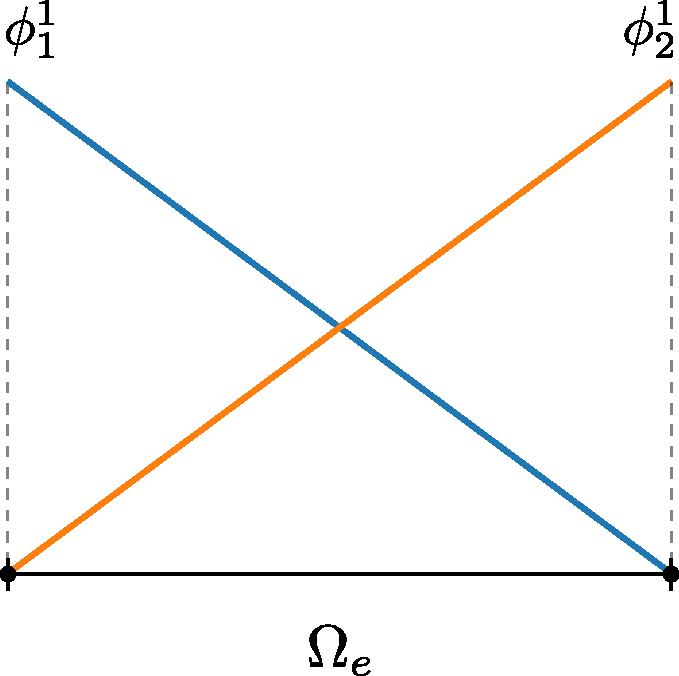
\includegraphics[width=0.4\linewidth]{img/elemento-base1}
	\caption{Polinômios de Lagrange de ordem $p=1$.}
	\label{f:lagrange-p1}
\end{figure}
\begin{figure}[h!]
	\centering
	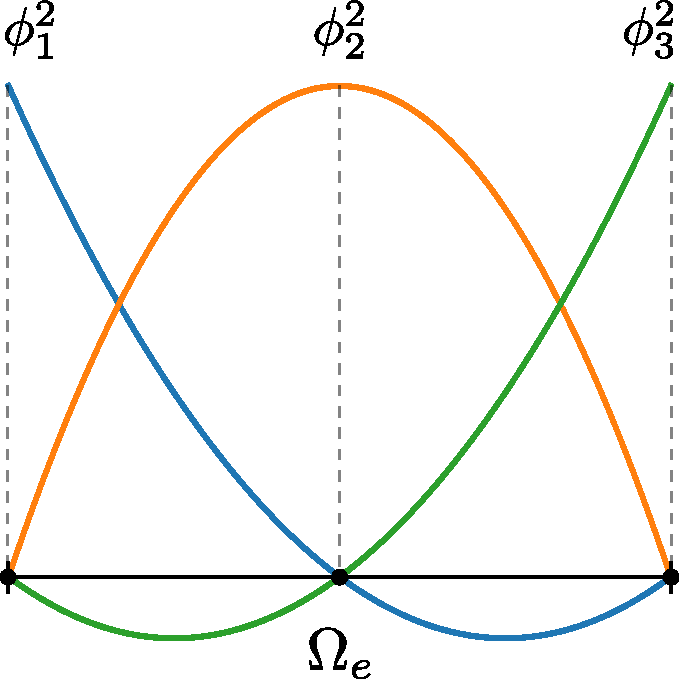
\includegraphics[width=0.4\linewidth]{img/elemento-base2}
	\caption{Polinômios de Lagrange de ordem $p=2$.}
	\label{f:lagrange-p2}
\end{figure}
\begin{figure}[h!]
	\centering
	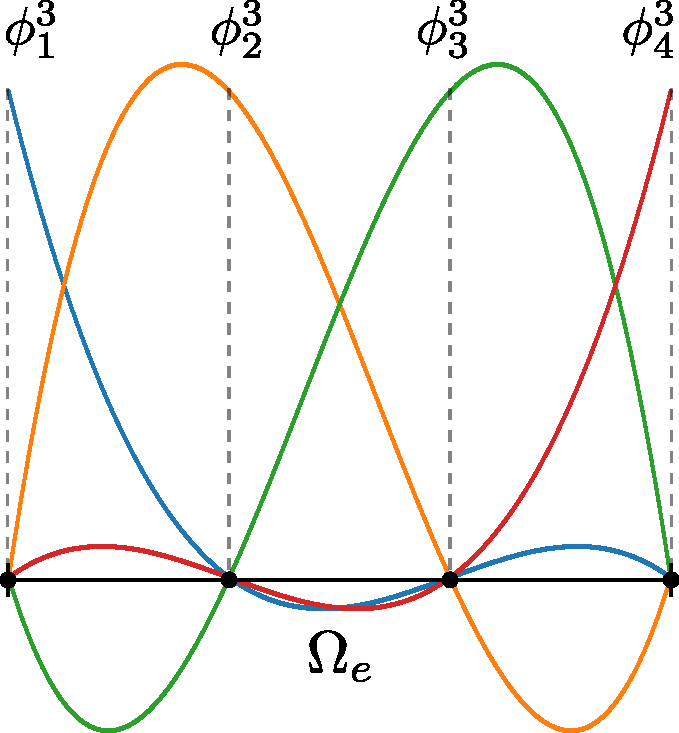
\includegraphics[width=0.4\linewidth]{img/elemento-base3}
	\caption{Polinômios de Lagrange de ordem $p=3$.}
	\label{f:lagrange-p3}
\end{figure}

A partir destas discretizações é possível aproximar a solução $u$ por uma combinação linear de uma base de Lagrange com coeficientes, obtendo-se $u_h$:	
\begin{equation}
	\begin{array}{l}
	\displaystyle
	u(x) \approx u^h(x) = \sum_{i=1}^{p+1} \psi_{i} \phi^p_i(x) , \enspace \psi_{i} \in \mathbb{R}
	\end{array}
	\label{e:aproximacao0}
\end{equation}

Os métodos de elementos finitos são obtidos a partir da adoção de uma formulação fraca para a equação diferencial do problema e da discretização da variável de interesse e sua função de ponderação em cada elemento do domínio. Comumente os modelos recaem em resolução e sistemas de equações. Na formulação apresentada para o problema deste trabalho, obtém-se um equação de autovalores generalizados (Seção \ref{s:mef-barra-continuo}).



\end{document}